\section{V21 Optisches Pumpen}
\label{sec:V21}

\begin{itemize}
    \item Untersuchung von Übergängen bestimmter Energieniveaus in Rubidium-Isotopen
    \item Erlaubt Bestimmung von Lande-Faktoren, sowie Elektronen- und Kernspins
\end{itemize}

\textbf{Theorie:}
\begin{itemize}
    \item Elektronen in Atomen auf festen Energienieveaus
    \item Veränderung des Niveaus erfordert/emittiert exakten Energiewert
    \item Besetzung äußerer Niveaus temperaturabhängig: Boltzmann-Verteilung
    \item Verhältnis der Besetzungszahlen zweier Niveaus:
        \begin{equation}
            \frac{N_2}{N_1}=\frac{g_2}{g_1}\frac{\exp(\sfrac{W_2}{k_BT})}{\exp(\sfrac{W_1}{k_BT}}
        \end{equation}
    \item Mit den Energien $W_i$, und den Lande-Faktoren, die beschreiben, wieviele Zustände zu der entsprechenden Energie gehören
    \item optisches Pumpen ermöglicht das Erzeugen einer Abweichung davon, bis hin zur Besetzungsinversion
    \item so eine nicht thermische Verteilung ermöglicht induzieren von Übergängen, sodass Energien des entstehenden Lichtes gut vermessen werden können
    \item Verteilung der Elektronen auf Energieniveaus folgt Auswahlregeln
    \item Magnetische Momente aus Gesamtdrehimpuls, Drehimpuls und Spin $\propto \sqrt{J(J+1)}$
    \item Moment aus Gesamtdrehimpuls präzediert um Gesamtdrehimpuls $J$
    \item $g_J$ ist abhängig von $J,S,L$
    \item Äußeres Magnetfeld verursacht Aufspaltung der Energieniveaus (Zeeman-Effekt)
       \begin{figure}[htb]
          \centering
          \includegraphics[width=0.75\textwidth]{figures/aufspaltung.jpg}
          \caption{Aufspaltung der Energieniveaus innerhalb eines Atomes. Dargestellt
                    sind die Feinstrukturaufspaltung durch den Elektronenspin, die
                    Hyperfeinstrukturaufspaltung durch den Kernspin, sowie die Zeeman-Aufspaltung
                    durch ein äußeres Magnetfeld.}
        \end{figure}
\end{itemize}

\textbf{Optisches Pumpen:}
\begin{itemize}
    \item Betrachte System ohne Kernspin mit zwei angeregten, sowie einem Grundzustand
      \begin{figure}[htb]
          \centering
          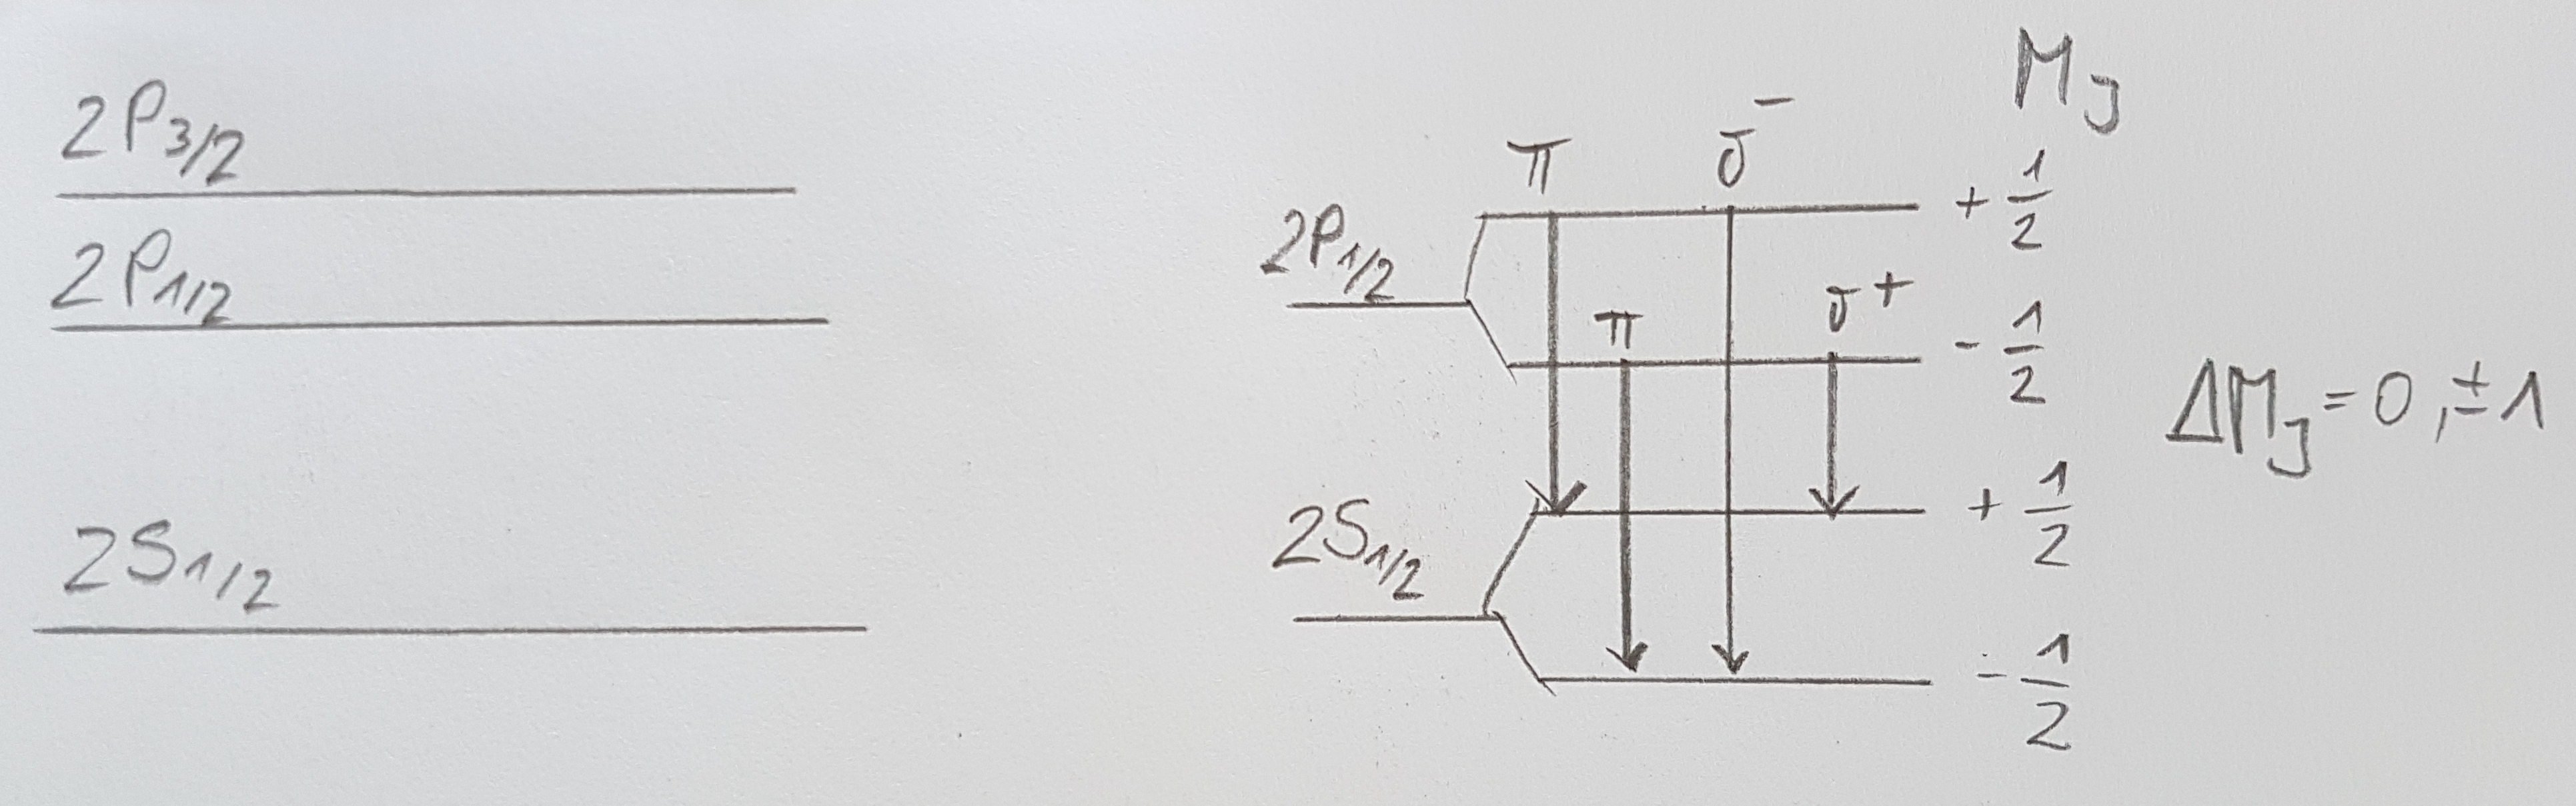
\includegraphics[width=0.75\textwidth]{figures/beispiel.jpg}
        \end{figure}
    \item In der Zeeman-Aufspaltung entstehendes Licht besitzt bestimmte Polarisationen
    \item Die $\sigma^\pm$ Linien sind rechts- bzw. linkszirkular polarisiert und erscheinen nur parallel zum Magnetfeld
    \item Die $\pi$-Linien sind linear polarisiert und werden nicht parallel zum B-Feld emittiert
    \item Licht einer Spektrallampe auf $D_1$-Filter und Polarisationsfilter, sodass rechtszirkularpolarisiertes $D_1$-Licht
    \item Einziger Übergang dann $^2S_{\sfrac{1}{2}}$ zu $^2P_{\sfrac{1}{2}}$, bzw rückwärts durch Emission
    \item Bei der Emission werden allerdings beide $^2S_{\sfrac{1}{2}}$ Zeeman-Niveaus besetzt, sodass das $M_J = -\sfrac{1}{2}$ langsam leergepumpt wird
    \item Daraus folgt eine Besetzungsumkehr im S-Niveau, die sich in der Transparenz der Dampfzelle widerspiegelt
    \item je weniger Elektronen im unteren Niveau sind, und angeregt werden können, desto durchsichtiger der Dampf
    \item 2 Prozesse: spontane Emission / angeregte Emission
    \item spontane Emission $\propto \nu^3$. Hierbei quasi nur induziert, da niedrige Energie
    \item Energiedifferenzen in Zeeman abhängig von B-Feld: $h\nu = g_J\mu_BB\upD M_J$
    \item Bei angelegtem B-Feld automatisch Besetzungsinversion, allerdings nur bis $B_m = \frac{4\pi m_0}{e_0g_J}\nu$, dann induzierte Emission
    \item bei stärkeren Magnetfeldern neben WW der magnet. Momente mit äußerem Magnetfled auch Effekt zwischen den Momenten untereinander wichtig
    \item bei schnell ein oder ausgeschalteten Magnetfeldern \textbf{transiente Effekte}: gedämpfte Schwingung bei Messung der Transparenz
    \item Grund: Präzession des magnet. Momentes (klassisch: mit Larmor-Frequenz)
    \item Frequenz ermöglicht Bestimmung des Isotopenverhältnisses in Lampe, da Periodendauer spezifisch für Isotop
\end{itemize}

\textbf{Durchfürung:}
\begin{itemize}
    \item Licht einer Rubidiumlampe über Linse fokussiert und parallelisiert
    \item $D_1$-Filter filtert $\SI{794,8}{\nano\meter}$ Linie heraus
    \item Filter besteht aus Dielektrikum der Dicke $d$ und Brechungsindex $n$, das von einer reflektierenden Schicht umgeben ist
    \item Mehrfache Reflektion von einfallendem Licht sorgt dafür, dass Wellenlängen der Größe
        \begin{equation}
            m\cdot \lambda_m = 2nd+\frac{\lambda}{2}
        \end{equation}
        konstruktiv interferiert
    \item Dann lineare Polarisation durch Filter um dann mit $\sfrac{\lambda}{4}$-Plättchen zirkular gemacht zu werden.
    \item \textbf{$\sfrac{\lambda}{4}$-Plättchen:} aus anisotropem Material bestehende Verzögerungsvorrichtung. Verzögert Licht entlang zweier Achsen unterschiedlich stark, sodass ein gewünschter Phasenunterschied erzeugt werden kann. Für linear zu zirkular muss Phasenunterschied $\sfrac{\pi}{2}$ sein
    \item Licht fällt dann auf Dampfzelle, die elktrisch beheizbar ist (Druckregulation/breitere thermische Verteilung)
    \item Zelle von zwei Helmholtzspulenpaaren umgeben. Nord-Süd Ausrichtung um horizontal und eine Spule um vertikal das Magnetfeld ausgleichen zu können
    \item dann mit zweiter Spule niederfrequentes B-Feld anlegen + Decke um Licht abzuschirmen
    \item Sägezahnspannung an Spulenpaar und Untersuchung der dips bei verschiedenen Frequenzen
    \item dann Rechteckspannung variierender Frequenzen um Überschwingen zu untersuchen (Frequenz bestimmen)
\end{itemize}

\textbf{Auswertung:}
\begin{itemize}
    \item Lande-Faktoren $g_F$ aus lokalem Minimum für verschiedene Frequenzen der Sweep-Spule
    \item lineare Regression des Magnetfeldes gegen die Frequenz
    \item aus $g_F$ lässt sich $g_J$ und dann der Kernspin $I$ bestimmen: $I=\frac{g_J}{2g_F}-\frac{1}{2}$
    \item $I_{87} = 1,520\,\pm\,0,016$ (soll $\sfrac{3}{2}$) und $I_{85} = 2,505\,\pm\,0,013$ (soll $\sfrac{5}{2}$)
    \item Isotopenverhältnis wird aus Amplitudenunterschied der Transparenzminima bei Hochfrequenzmessung bestimmt
    \item $\frac{N(85)}{N(87)}\approx 2$
\end{itemize}
